\documentclass[conference]{IEEEtran}
\IEEEoverridecommandlockouts
\usepackage{cite}
\usepackage{amsmath,amssymb,amsfonts}
\usepackage{algorithmic}
\usepackage{graphicx}
\usepackage{textcomp}
\usepackage{xcolor}
\usepackage{booktabs}
\usepackage{multirow}
\usepackage{url}
\def\BibTeX{{\rm B\kern-.05em{\sc i\kern-.025em b}\kern-.08em
    T\kern-.1667em\lower.7ex\hbox{E}\kern-.125emX}}
\begin{document}

\title{Work-in-Progress: Joint Optimization of Hierarchical IDK Cascades using a Memetic Genetic Algorithm with Simulated Annealing\\
\thanks{Work-in-Progress paper.}
}

\author{
\IEEEauthorblockN{Athan Chee}
\IEEEauthorblockA{\textit{The John Cooper School} \\
Spring, Texas, USA \\
athan5057@gmail.com}
\and
\IEEEauthorblockN{Samarthraj Arehally Basavaraj}
\IEEEauthorblockA{\textit{Cy-Fair High School} \\
Cypress, Texas, USA \\
samarthrajbasavaraj@gmail.com}
\and
\IEEEauthorblockN{Lucas Borgarello}
\IEEEauthorblockA{\textit{Strake Jesuit} \\
Katy, Texas, USA \\
lucasborgarello@gmail.com}
\and
\IEEEauthorblockN{Albert M. K. Cheng}
\IEEEauthorblockA{\textit{Department of Computer Science} \\
\textit{University of Houston}\\
Houston, TX 77004, USA \\
cheng@cs.uh.edu}
\and
\IEEEauthorblockN{Thomas Carroll}
\IEEEauthorblockA{\textit{Department of Computer Science} \\
\textit{University of Houston}\\
Houston, TX 77004, USA \\
tcarroll@uh.edu}
}

\maketitle

\begin{abstract}
Cyber-physical systems that host learning-enabled classifiers must reduce expected latency while meeting an accuracy contract on limited processors.
Hierarchical IDK cascades exploit a class taxonomy with intermediate routers, specialized branches, and a deterministic fallback~$K_{\mathrm{det}}$~\cite{baruah2025timely}.
Prior hierarchical work optimizes cascade layout~$S$ at fixed registry confidence cutoffs; prior cascade tuning jointly searches order and thresholds only on \emph{linear} chains~\cite{chellapilla2006combining,markatopoulou2016ordering}.
We jointly search hierarchical layout~$S$ and per-occurrence IDK thresholds~$H$ under a validation accuracy floor~$\alpha$, using a memetic genetic algorithm with an inner simulated-annealing threshold search, minimizing expected latency~$\bar{C}$.
On M3N-VC h24 at $\alpha{=}0.98337$, memetic joint search reduces validation~$\bar{C}$ by $27.6$\,ms versus thresholds-only retuning of a fixed hierarchy and recovers cost within $0.69$\,ms of an exhaustive layout baseline at $9\%$ of the layout budget.
\end{abstract}

\begin{IEEEkeywords}
Hierarchical IDK Cascades, Real-Time Systems, Memetic Algorithm, Simulated Annealing
\end{IEEEkeywords}

\section{Introduction}
Cyber-physical systems increasingly integrate deep classifiers under tight compute budgets, so average classification latency must fall without collapsing accuracy~\cite{abdelzaher2023scheduling,baruah2021optimal}.
IDK (``I don't know'') cascades address this trade-off: each classifier~$K_i$ returns a label only if its confidence meets a cutoff~$H_i$; otherwise it returns IDK and the input proceeds to a successor, ending at a deterministic fallback~$K_{\mathrm{det}}$~\cite{wang2018idk,abdelzaher2023scheduling}.
Real-time work synthesizes cascade order to minimize expected time, including robust and fault-tolerant variants~\cite{baruah2021optimal,baruah2023robust,baruah2024fault}.

Hierarchical IDK cascades extend the linear chain with intermediate classifiers~$K_I$ (e.g., COUPE/SUV/BACKGROUND), specialized classifiers~$K_\ell$, and globals~$K_\phi$ that may appear on multiple branches~\cite{baruah2025timely}.
Timely Classification of Hierarchical Classes optimizes cascade \emph{structure} for fixed, precision-calibrated registry thresholds (their Table~IV reports required-precision targets such as $0.90$/$0.95$, not the stored cutoffs themselves)~\cite{baruah2025timely}.
That contract differs from minimizing empirical $\bar{C}$ subject to an accuracy floor~$\mathrm{Acc}\!\ge\!\alpha$.
Related UH WIPs improve \emph{online} skip decisions in linear ImageNet cascades~\cite{nguyen2024probabilistic,katikaneni2025rfskip}; we instead \emph{offline jointly design} hierarchical banks $(S,H)$ on M3N-VC under an Acc floor.

\textbf{Contribution.}
We evaluate bilevel joint optimization of layout~$S$ and per-occurrence thresholds~$H$ with a constrained memetic GA (outer) and simulated annealing (inner).
On h24, retuning~$H$ under $\alpha$ already helps, and jointly searching~$S$ further reduces~$\bar{C}$, approaching an exhaustive K1-free layout baseline within a fixed search budget.

The remainder of this paper is organized as follows:
\begin{itemize}
\item hierarchical setup and classifier bank on M3N-VC h24;
\item threshold optimization by simulated annealing on a fixed layout;
\item memetic joint search over layouts with inner SA;
\item Acc-floor experiments versus thresholds-only and exhaustive layout search.
\end{itemize}

\section{Methodology}

\begin{figure}[t]
\centering
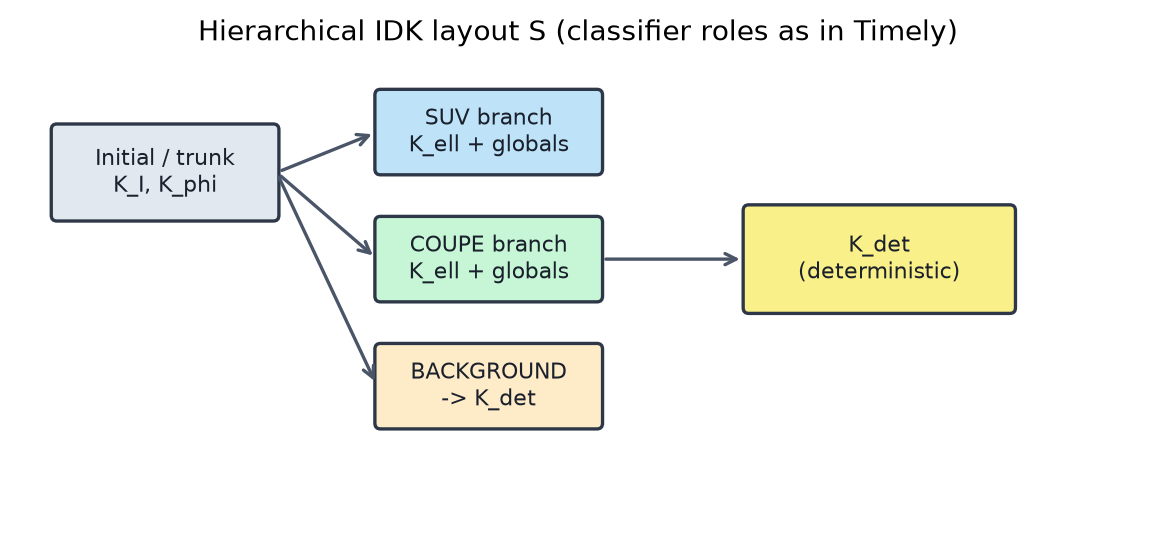
\includegraphics[width=\columnwidth]{figures/fig_hierarchy.png}
\caption{Hierarchical layout~$S$: an initial trunk of intermediate/global classifiers routes into specialized branches, then~$K_{\mathrm{det}}$. The same~$K_i$ may appear in multiple places; each occurrence may carry its own~$H$.}
\label{fig:hierarchy_example}
\end{figure}

\begin{table*}[t]
\centering
\renewcommand{\arraystretch}{1.15}
\setlength{\tabcolsep}{5pt}
\begin{tabular}{r|cc|cc|c|cc|c}
\toprule
Classifiers
& \multicolumn{2}{c|}{Intermediate}
& \multicolumn{2}{c|}{Global}
& \multicolumn{1}{c|}{SUV}
& \multicolumn{2}{c|}{COUPE}
& \multicolumn{1}{c}{Fallback} \\
& $K_0$ & $K_1$
& $K_2$ & $K_3$
& $K_4$
& $K_5$ & $K_6$
& $K_{\mathrm{det}}$ \\
\midrule
Modality
& Both & Both & Both & Both & Acoustic & Acoustic & Both & --- \\
Parameter count
& 141{,}379 & 354{,}827 & 141{,}637 & 1{,}218{,}173 & 37{,}858 & 37{,}858 & 141{,}250 & --- \\
Calibrated $H_i$
& 0.712 & 0.558 & 0.613 & ${\approx}0$ & 0.502 & 0.691 & 0.916 & --- \\
Non-IDK Acc
& 91.7\% & 93.4\% & 84.2\% & 93.9\% & 94.9\% & 85.5\% & 88.0\% & 100\% \\
Success rate ($1{-}p_{\mathrm{IDK}}$)
& 91.3\% & 96.0\% & 86.3\% & 100\% & 99.9\% & 71.2\% & 74.0\% & 100\% \\
Mean exec.\ time (ms)
& 1.967 & 8.791 & 6.711 & 12.676 & 2.264 & 2.301 & 1.882 & 10{,}000 \\
\bottomrule
\end{tabular}
\caption{Classifier bank from our registry on h24. Roles and parameter-count targets follow Timely~\cite[Table~IV]{baruah2025timely}; reported $H_i$ are \emph{calibrated} cutoffs, not the paper's required-precision targets $0.90$/$0.95$. $K_{\mathrm{det}}$ is the modeled $10{,}000$\,ms always-correct fallback~\cite{baruah2025timely}.}
\label{tab:classifiers}
\end{table*}

\textbf{Notation.}
$H_i$ is the softmax confidence cutoff for IDK; $\alpha$ is the validation accuracy floor; $S$ is the hierarchical layout; $\bar{C}$ is expected cascade latency (objective); $C_i$ denotes WCET used only in deadline/feasibility discussion and is not interchangeable with~$\bar{C}$.

\textbf{Data and training.}
We reproduce Timely's public protocol on M3N-VC h24~\cite{m3nvc2025zenodo,li2025restoreml,baruah2025timely}: acoustic ($1.6$\,kHz) and seismic ($200$\,Hz) streams, $2$\,s STFT windows, four base vehicles (Mustang, MX-5, CX-30, GLE~350) under COUPE/SUV plus BACKGROUND.
Classifier training uses run0,2,4,6 and $80\%$ of run8; held-out runs support testing.
Cascade optimization uses an $80\%$ blocked split of run1,3,5,7,9 (seed~$0$); the remaining $20\%$ is \emph{report-only} and never used for tuning.
We train seven spectrogram CNNs $K_0$--$K_6$ with roles and parameter counts aligned to Timely~\cite[Table~IV]{baruah2025timely} (globals on five base/BACKGROUND labels; identifiers on SUV/COUPE/BACKGROUND; specialized on two base classes).
After freezing the CNNs we cache per-window labels and confidences.
$K_{\mathrm{det}}$ is the artificial $10{,}000$\,ms deterministic fallback of~\cite{baruah2025timely}, not a measured Jetson WCET.
Table~\ref{tab:classifiers} summarizes the bank; Fig.~\ref{fig:hierarchy_example} sketches legal layouts.

\textbf{Threshold optimization (fixed~$S$).}
Given a layout, we adapt simulated annealing on a quantile confidence grid~\cite{chellapilla2006combining,li2025restoreml}: energy penalizes Acc below~$\alpha$, then minimizes empirical~$\bar{C}$ on the cached outcome table (no live DNN in the inner loop).
Repeated occurrences of the same~$K_i$ receive independent thresholds.
Default inner budget: $8$k iterations, $50$ quantiles.
For reliability we take best-of-$10$ independent SA trials when scoring layouts for joint search.

\begin{figure*}[t]
\centering
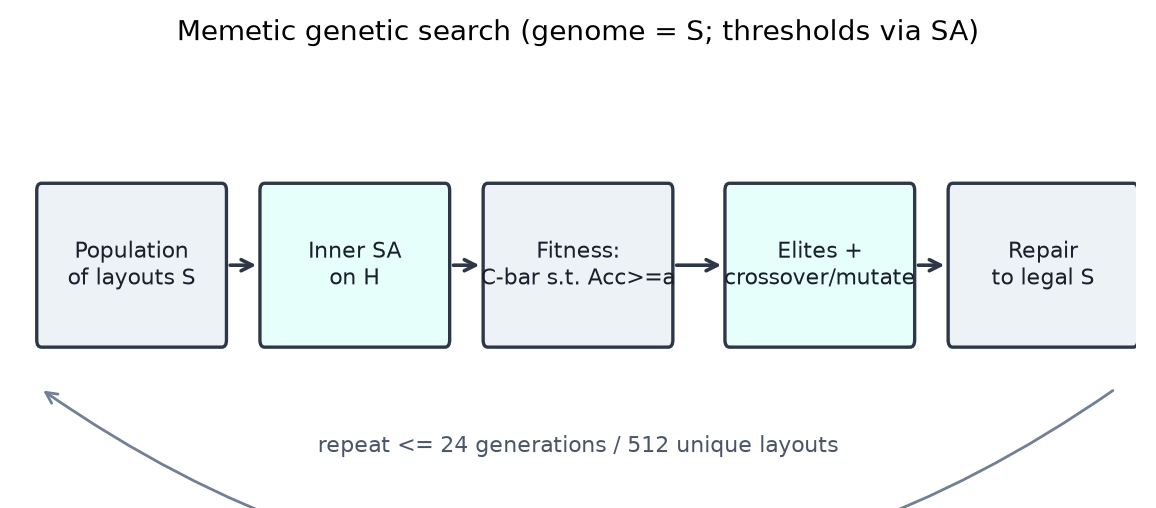
\includegraphics[width=0.92\textwidth]{figures/fig_genetic.png}
\caption{Memetic genetic algorithm: genomes encode layout~$S$ only; each candidate is scored by inner SA on~$H$.}
\label{fig:genetic_diagram}
\end{figure*}

\textbf{Memetic joint optimization.}
We use a memetic GA~\cite{moscato1989memetic} so the outer search explores layouts while SA polishes~$H$ (Fig.~\ref{fig:genetic_diagram}).
A genome is the cascade layout only---thresholds are never genes.
Initial population: $31$ random legal genomes plus a guaranteed $K_3{\to}K_{\mathrm{det}}$ seed ($32$ total).
After SA scoring, the best~$4$ elites advance.
Immigration rate $20\%$ inserts unseen random genomes; remaining slots use tournament selection of size~$2$, then crossover and mutation (both rate~$80\%$).
Crossover inherits a branch from one parent ($70\%$) or mixes shared classifiers with uniform keep probability on exclusive ones ($30\%$).
Mutation picks a branch (main trunk weight~$40\%$; specialized branches share the rest) and applies randomization, insert, delete, replace, swap, or relocate of a legal classifier.
A repair step enforces legality:\footnote{Main trunk $\subseteq$ globals$\cup$intermediates; each specialized branch lists only specialized/global classifiers not already executed on the trunk; every path ends in~$K_{\mathrm{det}}$.}
Search stops at $24$ generations or $512$ unique layouts (vs.\ $5545$ exhaustive K1-free layouts under the same grammar).

\section{Experiments and Results}

We compare three design methods under the same validation Acc floor $\alpha{=}0.98337$ on h24: (i)~thresholds-only SA on a frozen hierarchical layout; (ii)~memetic joint $(S,H)$ search (budget $512$ layouts); (iii)~exhaustive outer layout search with the same inner SA (upper reference).
Holdout Acc/cost are reported only.
Live Jetson Nano end-to-end timing of the winning banks is deferred to future work; numbers below are empirical~$\bar{C}$ on cached outcomes, not WCET claims.

\begin{figure}[t]
\centering
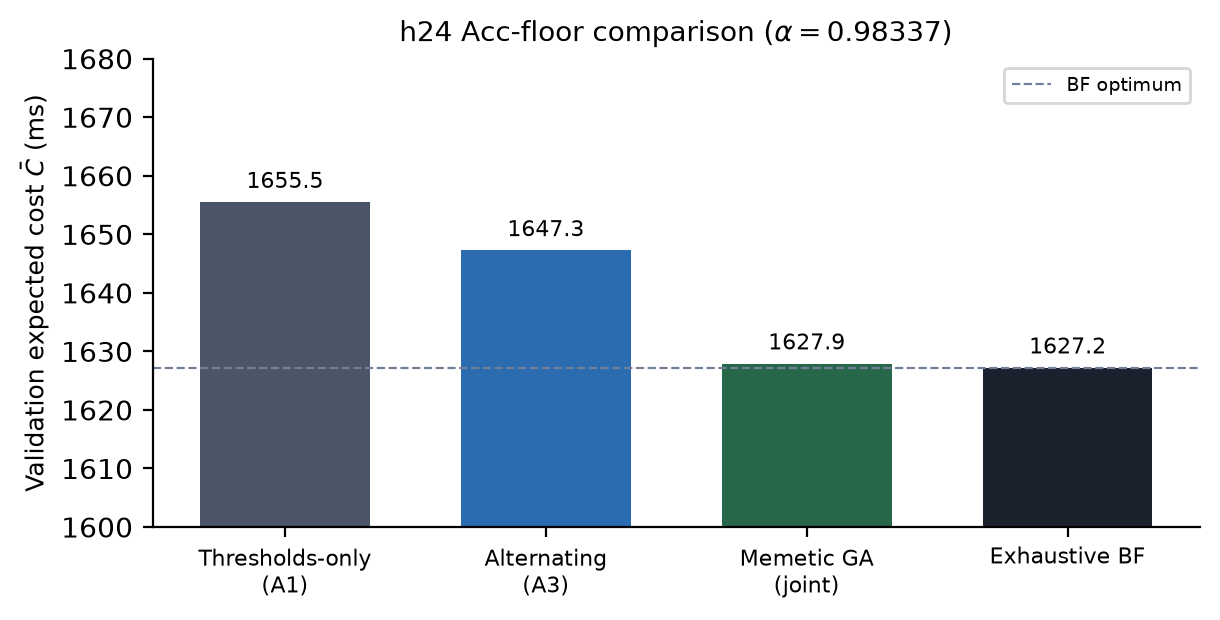
\includegraphics[width=\columnwidth]{figures/fig_finding1_cost.png}
\caption{Validation expected cost~$\bar{C}$ under Acc~$\ge\alpha{=}0.98337$ on h24. Memetic joint search approaches the exhaustive layout baseline and beats thresholds-only.}
\label{fig:finding1}
\end{figure}

\begin{table}[t]
\centering
\caption{Acc-floor bakeoff on h24 ($\alpha{=}0.98337$). Holdout unused for tuning.}
\label{tab:bakeoff}
\begin{tabular}{lcccc}
\toprule
Method & Joint? & Val Acc & Val $\bar{C}$ (ms) & Holdout $\bar{C}$ (ms) \\
\midrule
Thresholds-only (A1) & no & 0.9834 & 1655.51 & 1557.62 \\
Alternating (A3) & yes & 0.9834 & 1647.27 & 1557.42 \\
Memetic GA (512) & yes & 0.9834 & 1627.92 & 1534.71 \\
Exhaustive BF (5545) & yes & 0.9834 & 1627.23 & 1530.94 \\
\bottomrule
\end{tabular}
\end{table}

Fig.~\ref{fig:finding1} and Table~\ref{tab:bakeoff} summarize the bakeoff.
Memetic joint search improves validation~$\bar{C}$ by $27.59$\,ms versus thresholds-only SA on the frozen hierarchy while meeting the same Acc floor, and sits $0.69$\,ms above the exhaustive layout optimum at about $9\%$ of the outer layout budget ($512/5545$).
Alternating block-coordinate search closes part of the gap but remains above the memetic/BF costs.
For context, an EXPAND layout evaluated at registry~$H_i$ (different Acc contract) yields table-model $\mathbb{E}[C]{\approx}1194.7$\,ms and runtime Acc~${\approx}95.6\%$ on $n{=}8826$ validation windows in our reproduction; Acc-floor retuning is required to reach $\alpha{=}0.98337$.

\section{Related Work}
IDK cascades were introduced as cost-aware deferral over pretrained models~\cite{wang2018idk}.
Real-time synthesis minimizes expected time under dependences, deadlines, robustness, and fault tolerance~\cite{abdelzaher2023scheduling,baruah2021optimal,baruah2023robust,baruah2024fault}.
Threshold search and joint order+threshold tuning exist for \emph{linear} cascades~\cite{chellapilla2006combining,markatopoulou2016ordering,li2025restoreml}.
Timely Classification formalizes hierarchical IDK with intermediate and specialized roles and optimizes structure for fixed registry thresholds~\cite{baruah2025timely}.
Probabilistic and random-forest skip WIPs improve online middle-stage skipping on linear ImageNet cascades~\cite{nguyen2024probabilistic,katikaneni2025rfskip}.
These lines leave open joint Acc-floor search of hierarchical layout~$S$ and per-occurrence~$H$, which this WIP targets.

\section{Conclusion and Future Work}
We jointly optimized hierarchical IDK layout~$S$ and thresholds~$H$ under Acc~$\ge\alpha$ via a memetic GA with inner SA.
On M3N-VC h24 at $\alpha{=}0.98337$, joint search reduced validation~$\bar{C}$ by $27.6$\,ms versus thresholds-only retuning and approached an exhaustive layout baseline within $0.69$\,ms at a $512$-layout budget.
Limitations: the outer search is approximate; outcomes are scene-specific (h24); $K_{\mathrm{det}}$ cost is modeled; Jetson live timing of winning banks is not yet reported.
Future work includes faster search (early screening, parallel workers), history-dependent specialized order, scene-aware bank swap, multi-feature deferral at routers, and SoC validation on NVIDIA Jetson Nano.

\bibliographystyle{IEEEtran}
\bibliography{citations}

\end{document}
